\chapter{veYjAcnxnika takaR - oMdu lekakx}

\qquad nananx mitarx maMjunAthf oLeLxya vidAyxvaMta. aSeTxV alalx budadhxvaMta, takaR cenAnxgi tiLididadx. oMdu shAleya gaNita meVSuTxrX. avara taragatiyalilx ipapxtetxraDu ($22$) vidAyxthiRgaLidadxru. avaralilx ibabxru vidAyxthiRgaLu bahaLa budidhxvaMtaru. AgAgegx parxshenxgaLanUnx keVLutitxdadxru. meVSuTxrX keVLida elalx lekakxgaLigU beVga utatxra heVLutitxdadxru. taragatiyalilx elalxra muMde avaribabxrigU benunxtaTaTxde beVre yAvudAdarU oMdu saMdaBaRdalilx avaribabxrigU bahumAna koDabeVkeMdu tiVmARnisidadxru. nAnu AgaleV heVLidadx mitarx meVSuTxrX taragatiyalilxdadx I elAlx ipapxtetxraDu ($22$) vidAyxthiRgaLige karxmavAgi $1$ riMda $22$ra varege saMKeyxyanunx koTuTx adeV karxmadalilx oMdu vaqtAtxkAradalilx nililxsidaru.

\vskip .1cm

tanage beVkAgidadx A ibabxru budidhxvaMtaranunx oMdariMda AraMBisida $5$ matutx $19$neya sAthxnadalilx vaqtatxdalilx nililxsidadxru. Iga oMdariMdaleV lekakxvanunx pArxraMBisi parxtiyoMdu mUraneya vidAyxthiRyanunx horage aTuTxtAtx baMdare konege ibabxru mAtarx uLiyutAtxre. avarige beVkAgidadx $5$ matutx $19$neya sAthxnada vidAyxthiRgaLige uLiyuvaMte bahumAna koDuvaMte heVge\break EpARTumADidadxru noVDi.

\vskip .1cm

$1$ riMda $22$ravarege vidAyxthiRgaLanunx ililx tiLisidaMte vaqtAtxkAradalilx nililxsidaru.

\eject

{\bf modalaneya AvatiR:} oMdariMda I lekakxvanunx pArxraMBisi parxti\-yoMdu\break mUraneya vidAyxthiRyanunx horage aTuTxtAtx baMdu, alilxMda punaH muMdu\-varisidare $21$neya sAthxnakekx nilulxtatxde.
\begin{figure}[H]
\centering
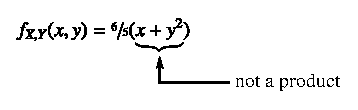
\includegraphics[scale=0.75]{src/figures/fig8.eps}
\end{figure}

\begin{figure}[H]
\centering
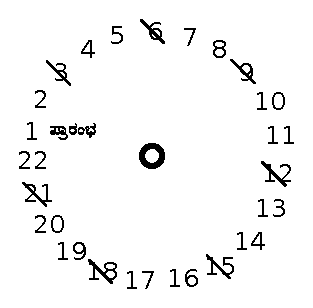
\includegraphics[scale=0.75]{src/figures/fig9.eps}
\end{figure}
 

modalaneya AvatiRyalilx horage vidAyxthiRgaLu $3$, $6$, $9$, $12$, $15$, $18$, $21$.

{\bf eraDaneya AvatiR:} uLida vidAyxthiRgaLanunx hiMdina sAthxnadaMteyeV vaqtAtxkAradalilx nililxsidaru.

$21$neya sAthxna konege horage aTiTxtutx. $22$riMda AraMBisi parxti mUraneya vidAyxthiRyanunx horage aTuTxtAtx baMdare $20$neya sAthxnakekx nilulxtatxde. 
\begin{figure}[H]
\centering
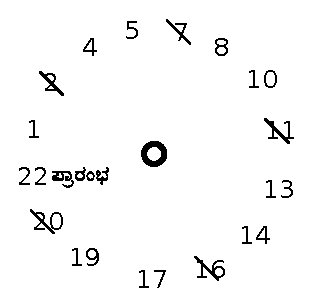
\includegraphics[scale=0.75]{src/figures/fig10.eps}
\end{figure}
eraDaneya AvatiRyalilx horage hoVguva vidAyxthiRgaLU $2$, $7$, $11$, $16$, $20$.

{\bf mUraneya AvatiR:} uLida vidAyxthiRgaLanunx hiMdina sAthxnadaMteyeV vaqtAtxkAradalilx nililxsidaru.

$20$ neya sAthxna horage aTiTxtutx. $22$riMda AraMBisi parxti mUraneya vidAyxthiRyanunx horage aTuTxtAtxbaMdare, $17$neya sAthxnakekx baMdu nilulxtatxde. 
\begin{figure}[H]
\centering
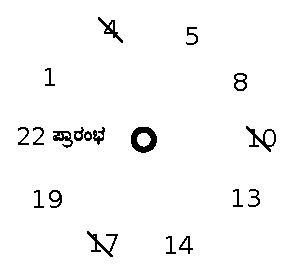
\includegraphics[scale=0.8]{src/figures/fig11.eps}
\end{figure}

mUraneya AvatiRyalilx horage hoVguva vidAyxthiRgaLu $4$, $10$, $17$ 

{\bf nAlakxneya AvatiR:} uLida vidAyxthiRgaLanunx hiMdina sAthxnadiMdaleV vaqtAtxkAra\-dalilx nililxsidaru.

$17$neya sAthxna horage aTiTxtutx. $19$riMda AraMBisi parxtiyoMdu mUraneya vidAyxthiRyanunx horage aTuTxtAtxbaMdare. $22$neya sAthxnakekx nilulxtatxde. 
%\fbox{\parbox{0.9\textwidth}{gaNitavanunx cenAnxgi aMtariVkarisikoMDavarige iMtaha moVjinATagaLanunx ADuvudu
   % sAdhayx. beVre yAva viSayadalUlx iMtaha kalapxnAtamxka caTuvaTike kaSaTx.}}
\begin{figure}[H]
\centering
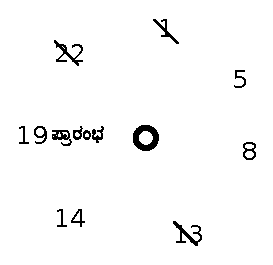
\includegraphics[scale=0.8]{src/figures/fig12.eps}
\end{figure}

nAlakxneya AvatiRyalilx horage hoVguva vidAyxthiRgaLu $1$, $13$, $22$.

{\bf aidaneya AvatiR:} uLida vidAyxthiRgaLanunx hiMdina sAthxnadiMdaleV vaqtAtxkAra\-dalilx nililxsidaru.

$22$neya sAthxna horage aTiTxtutx. $5$riMda AraMBisi parxti mUraneya vidAyxthiRyanunx horage aTuTxtAtx baMdare
\begin{figure}[H]
\centering
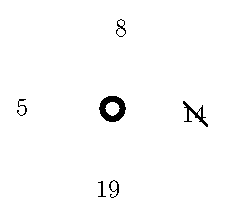
\includegraphics[scale=0.8]{src/figures/fig13.eps}
\end{figure}

aidaneya AvatiRyalilx horage hoVguva vidAyxthiR $14$.

{\bf Araneya AvatiR:} uLida vidAyxthiRgaLanunx hiMdina sAthxnadiMdaleV vaqtAtxkAra\-dalilx nililxsidaru.

$14$neya sAthxna horage aTiTxtutx. $19$riMda AraMBisi parxtiyoMdu mUraneya vidAyxthiRgaLanunx horage aTuTxtAtx baMdare $19$ matutx $5$ uLiyutatxde. 
\begin{figure}[H]
\centering
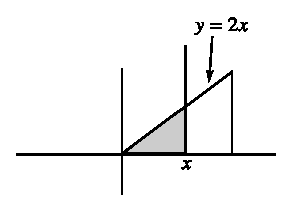
\includegraphics[scale=0.8]{src/figures/fig14.eps}
\end{figure}

Araneya, AvatiRyalilx horage hoVguva vidAyxthiR $8$.

Iga konege horage kaLuhisida meVle konege $5$ matutx $19$neya sAthxnada ibabxru vidAyxthiRgaLu mAtarx uLidaru.

meVSuTxrX maMjunAthf avarige beVkAgidadx $5$ matutx $19$neya vidAyxthiRgaLige bahumAna niVDidaru. avara takaR heVgide noVDi! idara kAraNavanunx niVveV Uhisi.
